\documentclass[11pt]{article}


\setlength{\parindent}{0pt}
\usepackage{xltxtra}
\usepackage{hyperref}
\hypersetup{hidelinks}
\usepackage{url}
\urlstyle{tt}
\usepackage{xcolor}
\definecolor{CVBlue}{RGB}{23,110,191}
\usepackage{calc}
\usepackage{graphicx}
\usepackage{tikz}
\usetikzlibrary{calc}
\usepackage{fontspec}
\usepackage{xeCJK}
\usepackage{enumitem}
\CJKsetecglue{} %% 取消中文与数字之间的间隙


%% 主文档字体设置
\setmainfont[
    Path = fonts/Main/,
    Extension = .otf,
    BoldFont = texgyretermes-bold.otf, % 加粗字体
]{texgyretermes-regular.otf} % 正文字体

% 中文字体设置
\setCJKmainfont[
    Path = fonts/hansans/,
    Extension = .ttf,
    BoldFont = NotoSansSC-Bold.ttf, % 加粗字体
]{NotoSansSC-Regular.otf} % 正文字体


\usepackage{relsize}
\usepackage{xspace}

% 使用 fontawesome（部分图标）
\usepackage{fontawesome}

% A4纸，上下左右边距
\usepackage[
    a4paper,
    left=1.2cm,
    right=1.2cm,
    top=1.5cm,
    bottom=1cm,
    nohead
]{geometry}

\renewcommand{\baselinestretch}{1.5} % 行间距设为1.5

\usepackage{titlesec}
\usepackage{enumitem}
\setlist{noitemsep} % 取消列表项间的额外间距
%\setlist{nosep} % 取消所有垂直间距
\setlist[itemize]{topsep=0.25em, leftmargin=*}
\setlist[enumerate]{topsep=0.25em, leftmargin=*}

% --- 用于控制【不同项目之间】的垂直距离 ---
\newlength{\interProjectSpacing}
\setlength{\interProjectSpacing}{0.9em} % <--- 在此调整项目之间的距离
\newcommand{\projectsep}{\vspace{\interProjectSpacing}}

% --- 用于控制【项目标题】与下方【项目描述】的距离 ---
\newlength{\intraProjectTitleSep}
\setlength{\intraProjectTitleSep}{0.4em} % <--- 在此调整标题和描述的距离
\newcommand{\titlebreak}{\\[\intraProjectTitleSep]}

% --- 用于控制【项目描述】与下方【要点列表】的距离 ---
\newlength{\intraProjectListTopSep}
\setlength{\intraProjectListTopSep}{0.2em} % <--- 在此调整描述与列表的距离

% =======================================================================


\titleformat{\section}         % 定制 \section 命令
{\large\bfseries\raggedright} % 将 section 标题设置为大号、粗体且左对齐
{}{0em}                      % 可用于为所有 section 添加前缀（如“章节...”）
{}                           % 可用于在标题前插入代码
[{\color{CVBlue}\titlerule}]  % 在标题后插入一条横线
\titlespacing*{\section}{0cm}{*1.6}{*1.2}



\begin{document}
\pagenumbering{gobble}

%%%% 利用tikz来定位照片（简历中未提供照片，已注释；如需照片，将照片命名为 avatar.jpg 放入本目录并取消下面三行的注释）
%\begin{tikzpicture}[remember picture, overlay]
%    \node[anchor = north east] at ($(current page.north east)+(-2cm,-1.2cm)$) {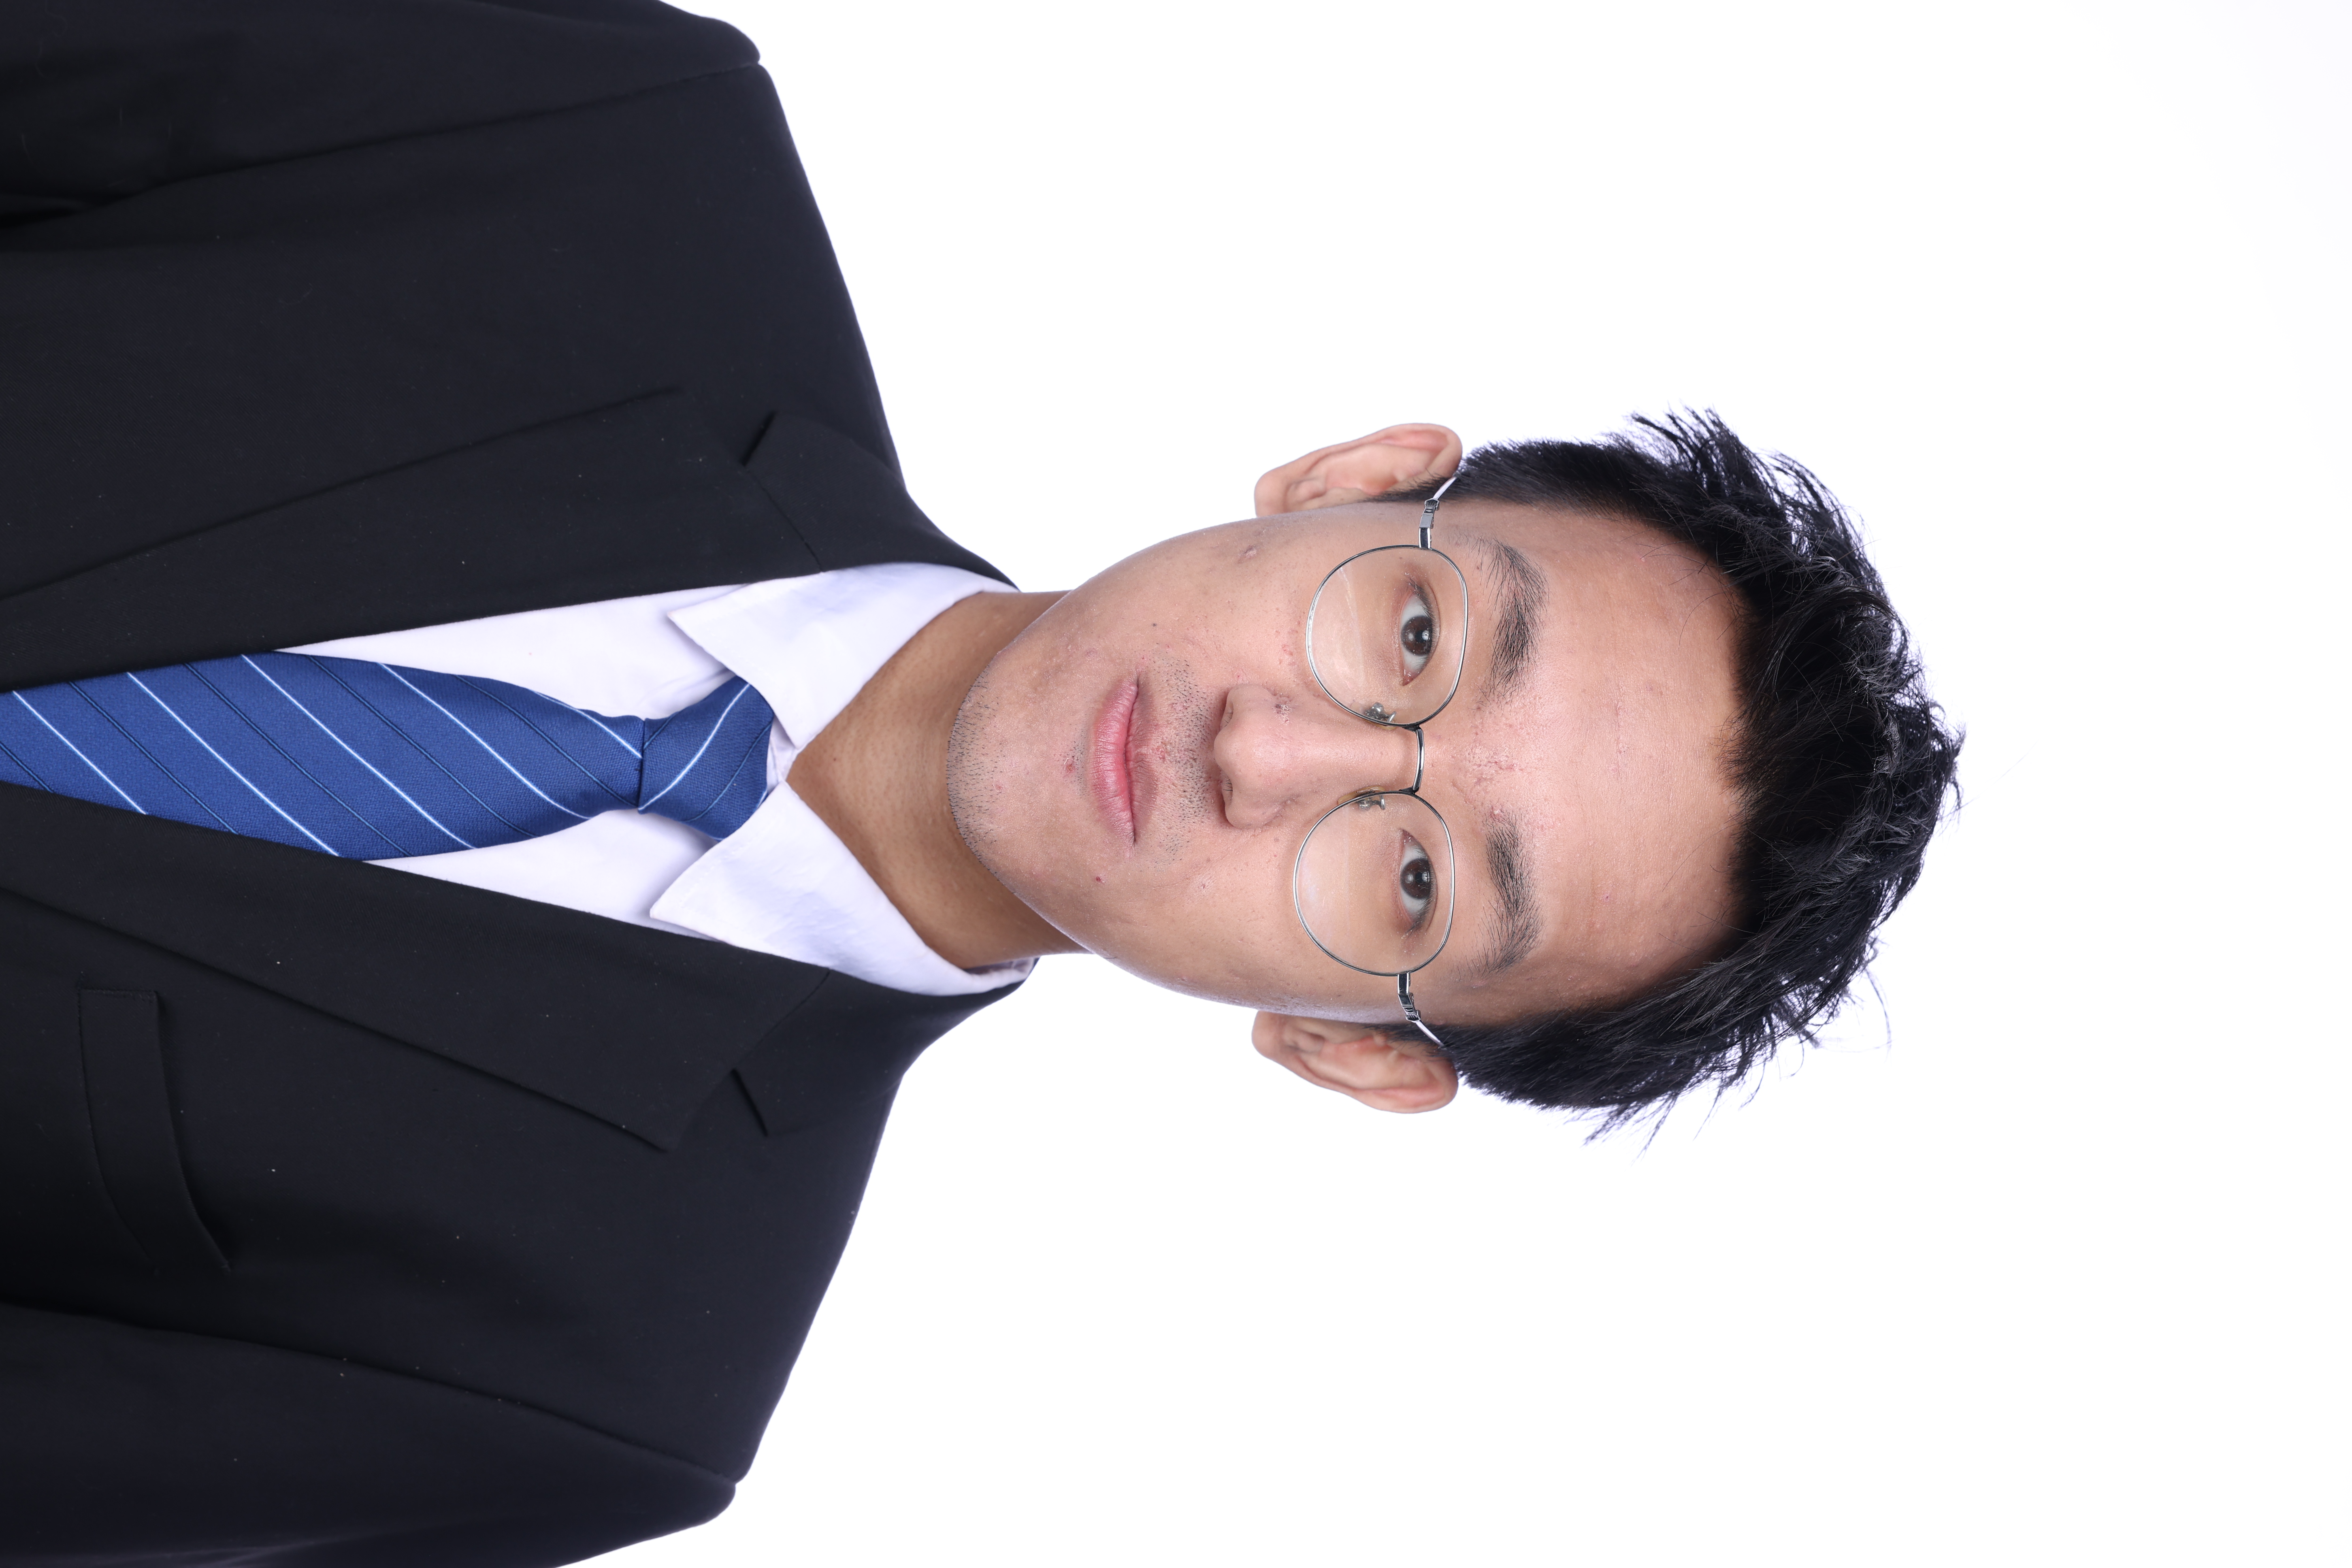
\includegraphics[height=3cm]{avatar.jpg}};
%  \end{tikzpicture}%
  %%%% 利用tikz来定位学校Logo，这里只在第一页显示
  \begin{tikzpicture}[remember picture, overlay]
    \node[anchor = north west] at ($(current page.north west)+(0.5cm,+1.0cm)$) {\includegraphics[height=6cm]{zju.png}};
  \end{tikzpicture}%
\centerline{\LARGE\bfseries{李硕}}

\vspace{5mm}
%\centerline{\normalsize{求职意向：大模型 / Agent 应用开发工程师（2027 届校招）}}

\centerline{\normalsize{\faPhone\ 136-1413-3375 \quad \faEnvelopeO\ \href{mailto:1050196454@qq.com}{1050196454@qq.com} \quad 现居地：浙江杭州}}

\centerline{\normalsize{学历：硕士 \quad 政治面貌：预备党员 \quad 生日：2002.03}}

\section{\makebox[\widthof{\faGraduationCap}][c]{\color{CVBlue}\faGraduationCap}\ 教育背景}
\textbf{浙江大学} \hfill 2024.09 -- 至今\\[0.5em] % 标题和正文间加一点距离
先进集成电路制造工程\quad 硕士研究生
\begin{itemize}[nosep]
    \item 研究方向：大模型与智能体（Agent）应用开发，人工智能辅助工业超声计量
\end{itemize}

\projectsep

\textbf{吉林大学} \hfill 2020.09 -- 2024.06\\[0.5em]
电子科学与工程\quad 本科
\begin{itemize}[nosep]
    \item 专业课程：机器学习、自然语言处理、计算机视觉、人工智能辅助集成电路制造、微电子器件物理
\end{itemize}

% 【投递前务必把公司名替换为可背书的真实公司名，详见随附的面试问答手册】
\section{\makebox[\widthof{\faBriefcase}][c]{\color{CVBlue}\faBriefcase}\ 实习经历}

\textbf{浙江睿朗信息科技有限公司} \hfill 2026.04 -- 2026.08\\[0.5em]
大模型应用开发实习生\quad 「领域专家」智能体工作站（Agent 运行底座 + 桌面客户端）从 0 到 1 搭建
\begin{itemize}[nosep, topsep=\intraProjectListTopSep]
    \item \textbf{方案设计与架构决策}：围绕“通用大模型缺乏领域知识、企业专属模型定制链路长门槛高”的痛点独立完成方案设计；第一版“采集—检索—生成”固定流水线验证后，针对其异常场景无法自适应的问题，将流程控制权从代码上移至大模型自主决策，重构为“Agent 运行底座—工具/技能体系—桌面客户端”三层架构。
    \item \textbf{Agent 底座开发}：手写目标驱动的工具调用调度主循环，配套三类质量门禁（工具协议校验、检索防重复空转的强制收敛、零结果与训练异常拦截）、失败反思反馈重注入与步数上限终态兜底；实现装饰器式工具注册中心，原子工具即插即用并自动导出 Function Calling 规范，沉淀 6+ 原子工具与 3 个复合技能（SOP）。
    \item \textbf{客户端与工程化}：独立交付 PyQt6 桌面客户端，支持多领域会话工作区、文献拖拽入库、5 家模型服务商配置与本地模型接入；采集、推理、训练三路任务子进程隔离，检索超时熔断与崩溃日志落盘；问答语料自动沉淀为训练集并设置最小语料量门禁，完成“语料沉淀—训练任务调度—进度监控—崩溃诊断”的微调链路工程化封装。
    \item \textbf{验证与成果}：在 7 个跨学科领域（含 4 个工科与 2 个人文历史方向）完成端到端验证，接入 arXiv、OpenAlex、Semantic Scholar 等 5 个学术数据源，累计入库结构化文献 184 篇、蒸馏领域问答语料 23 条，验证了架构的领域无关通用性与“一键生成文献综述”闭环可行性；全程 AI 辅助编码、沉淀 400 余页调试复盘日志。
\end{itemize}

\projectsep

\textbf{合作企业（高校横向课题）} \hfill 2025.09 -- 2026.06\\[0.5em]
算法实习生 \quad 工业超声波气体流量计周期跳变智能检测与消除
\begin{itemize}[nosep, topsep=\intraProjectListTopSep]
    \item 跨 9 个月完成 -20℃～39℃ 多温度区间、6 个实验批次 20 余组工况的实气标定实验，独立负责数据采集与整理，构建实测样本 21,000 余组。
    \item 开展 200 余轮训练实验，独立定位仿真—实测域偏移问题（实测准确率仅 22.4\%），设计硬件噪声注入与物理机理驱动的稀缺样本合成方案，将实测准确率提升至 78.6\%（+56 个百分点）；最终模型在 21,652 组企业实测数据上平均误差 0.12 个计量周期，模型体积 3.5MB、CPU 单样本推理 2.3 毫秒，通过企业实测验证、达到工业部署标准。
\end{itemize}

\section{\makebox[\widthof{\faUsers}][c]{\color{CVBlue}\faUsers}\ 项目经历}

% --- 项目一：Agent 工程化（Docker / vLLM / MCP）---
\textbf{Agent 工程化实践：容器化交付、本地推理服务与 MCP 工具生态（个人项目）} \hfill 2026.09 \titlebreak
项目描述：在自研 Agent Harness 基础上补全“可交付、可部署”工程链路，独立完成容器化打包、本地推理服务部署与 MCP 标准协议工具接入。
\begin{itemize}[nosep, topsep=\intraProjectListTopSep]
    \item \textbf{容器化交付}：将 CLI 内核与桌面 GUI 解耦并作为容器 ENTRYPOINT（\texttt{python -u} 关闭块缓冲保证日志实时输出）；从完整环境手工裁剪依赖清单、剔除 PyQt6 等 GUI 依赖，镜像瘦身约 1GB；通过 \texttt{.dockerignore} 排除模型权重与密钥配置，使用 bind mount 与命名卷分离工作区、运行时配置与模型缓存；独立排查 WSL2 虚拟化组件缺失、数据盘占满导致运行时崩溃等环境问题并完成磁盘迁移。
    \item \textbf{本地推理服务}：基于 vLLM 官方镜像部署 Qwen2.5-1.5B-Instruct 的 OpenAI 兼容服务，实践 GPU 透传、共享内存、显存利用率与上下文长度等参数配置；定位并绕过 WSL2 平台 UVA 不可用的兼容性问题（切换 V1 runner），以卷挂载固化 torch.compile/CUDA graph 编译缓存、规避每次 30 分钟以上重复编译；验证同一套 OpenAI SDK 调用代码仅修改 \texttt{base\_url} 即在云端 API 与本地推理服务间零改动切换；理解 PagedAttention、连续批处理等推理优化机制。
    \item \textbf{MCP 工具协议}：基于 FastMCP 实现 MCP Server（装饰器注册工具，文档字符串与类型注解自动生成 JSON Schema），并编写 stdio 传输的 Client 完成 initialize 握手、tools/list 工具发现与 tools/call 调用全流程；理清 JSON-RPC 2.0 协议层与 stdio/HTTP 传输层的分工，以及 Function Calling（模型—底座）与 MCP（底座—工具服务）的分层边界。
\end{itemize}

\projectsep

% --- 项目二：端侧日程 Agent ---
\textbf{跨平台端侧智能日程提取智能体} \hfill 2026.07 -- 2026.08 \titlebreak
项目描述：针对智能助手多依赖电脑或云端部署、即时通讯中的日程信息易被遗漏的问题，以 AI 辅助编码方式独立完成需求拆解、开发与端侧联调，交付了一套运行于移动端的轻量级智能日程提取与系统级日历同步智能体技能。
\begin{itemize}[nosep, topsep=\intraProjectListTopSep]
    \item 结合移动端隐私特性，利用系统原生通知监听能力实现即时通讯消息的后台自动监听与过滤，不使用外挂或钩子手段。
    \item 设计防御性结构化输出约束，动态注入基准时间与星期信息，消除大模型在时间推算中的歧义与幻觉。
    \item \textbf{成果}：实现安卓与 iOS 端零人工干预静默同步；独立定位并解决大模型返回 Markdown 格式导致端侧解析崩溃的问题。
\end{itemize}

\projectsep

% --- 项目三：图像生成微调 ---
\textbf{特定角色一致性图像生成模型微调实践（独立项目）} \hfill 2026.08 -- 至今 \titlebreak
项目描述：为实现可控、高一致性的特定角色图像生成，以 AI 辅助编码方式独立完成从数据集构建、模型微调、推理测试到问题排查的完整闭环，验证了小样本个性化图像生成的工程可行性。
\begin{itemize}[nosep, topsep=\intraProjectListTopSep]
    \item 独立完成素材采集、筛选与标准化处理，按视角与表情动作姿态分类整理 30 余种场景，并逐张编写英文标注提示词，构建 34 张高质量训练集。
    \item 在 8GB 显存消费级显卡上完成训练环境搭建与显存优化，对比两套主流开源底模的微调效果；累计迭代 20 余轮参数实验、产出 178 张对比测试图，最终完成 70 轮微调，角色一致性与姿态可控性达到可稳定出图水平。
    \item 独立定位并解决底模离线加载失败、权重融合报错、显存溢出、生成角色特征崩坏等问题，在 AI 辅助编码产出幻觉代码的情况下独立完成任务拆解与调试闭环。
\end{itemize}

\section{\makebox[\widthof{\faCogs}][c]{\color{CVBlue}\faCogs}\ 技术栈}
\begin{itemize}[nosep]
    \item \textbf{大模型与 Agent：} 熟练 Python；掌握 Prompt Engineering、Function Calling、上下文/记忆管理、RAG 向量检索、结构化输出（JSON Schema）、质量门禁与反思重试等 Agent 核心机制；了解 SFT/LoRA 微调原理；理解 Transformer、注意力机制、tokenizer 等大模型基础原理
    \item \textbf{容器、部署与推理服务：} 掌握 Docker 镜像构建、依赖裁剪、卷挂载与 GPU 透传；具备 vLLM 本地推理服务部署与 OpenAI 兼容接口实践，了解 PagedAttention 与连续批处理；了解 MCP（JSON-RPC 2.0 / stdio）协议与 asyncio、多线程、多进程等并发模型；熟悉 Git、Linux 常用命令，了解 FastAPI 服务开发
    \item \textbf{深度学习：} 熟练使用 PyTorch；掌握 CNN、双向 GRU、多头注意力等时序建模方法；了解扩散模型（Illustrious-XL、Flux）图像微调全流程
    \item \textbf{AI Coding 实践：} 长期高频使用 AI 辅助编码工具独立完成 4 个完整项目，形成“需求拆解—代码生成—幻觉排查—运行验证—交付”的完整方法论，对 AI 生成代码的典型失效模式与分层验证策略有系统实践
\end{itemize}

\section{\makebox[\widthof{\faList}][c]{\color{CVBlue}\faList}\ 获奖情况}
\begin{itemize}
    \item 浙江大学集成电路学院优秀研究生 \hfill 2025
    \item 吉林大学校文体奖学金 \hfill 2021
    \item 吉林大学校三等奖学金 \hfill 2021
\end{itemize}

\end{document}
